% Misma curva f(I) = 4 sqrt(I), D = 6. Prestamista r_p = 10 %, prestatario r_d = 50 %.
% Tangencias: I_p = 3,306 (J_p = 2,69; G_p = 7,27) e I_d = 1,778 (J_d = 4,22; G_d = 5,33).
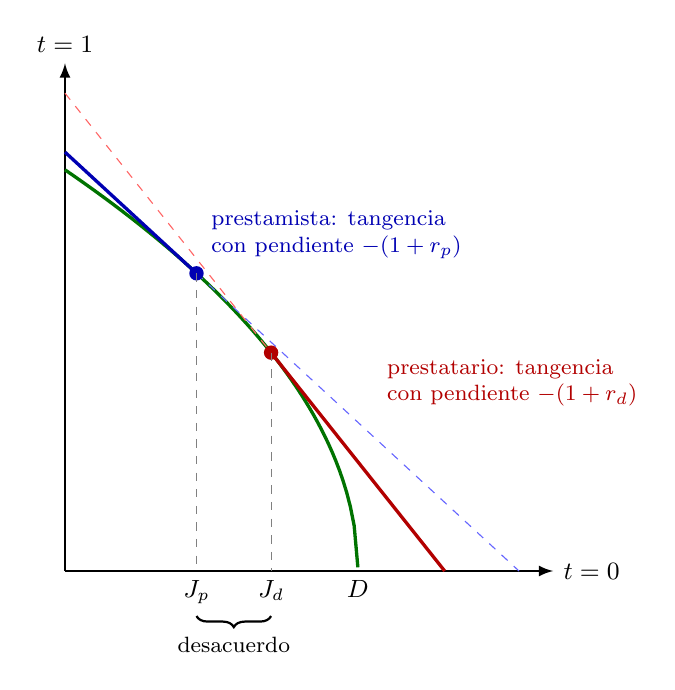
\begin{tikzpicture}[x=0.62cm, y=0.52cm, >=latex, font=\small]
  \draw[->, thick] (0,0) -- (10,0) node[right] {$t=0$};
  \draw[->, thick] (0,0) -- (0,12.4) node[above] {$t=1$};
  \draw[very thick, green!45!black, domain=0:6, samples=80] plot (\x,{4*sqrt(6-\x)});
  % Recta del prestamista (pendiente -1,1): solo el tramo hacia la izquierda (prestar)
  \draw[thin, dashed, blue!60] (2.694,7.27) -- (9.30,0);
  \draw[very thick, blue!70!black] (0,10.23) -- (2.694,7.27);
  % Recta del prestatario (pendiente -1,5): solo el tramo hacia la derecha (endeudarse)
  \draw[thin, dashed, red!60] (0,11.67) -- (4.222,5.333);
  \draw[very thick, red!70!black] (4.222,5.333) -- (7.778,0);
  \fill[blue!70!black] (2.694,7.27) circle (2.6pt);
  \fill[red!70!black] (4.222,5.333) circle (2.6pt);
  \draw[dashed, gray] (2.694,7.27) -- (2.694,0) node[below, black] {$J_p$};
  \draw[dashed, gray] (4.222,5.333) -- (4.222,0) node[below, black] {$J_d$};
  \node[below] at (6,0) {$D$};
  \node[blue!70!black, anchor=south west, font=\footnotesize, align=left] at (2.8,7.4) {prestamista: tangencia\\con pendiente $-(1+r_p)$};
  \node[red!70!black, anchor=west, font=\footnotesize, align=left] at (6.4,4.6) {prestatario: tangencia\\con pendiente $-(1+r_d)$};
  \draw[decorate, decoration={brace, mirror, amplitude=4pt}, thick] (2.694,-1.1) -- (4.222,-1.1)
     node[midway, below=4pt, font=\footnotesize] {desacuerdo};
\end{tikzpicture}
